\documentclass[11pt]{article}
\usepackage[margin=0.7in]{geometry}
\usepackage{multirow}
\usepackage {graphicx}
\usepackage[utf8x]{inputenc} % указать кодировку русского текста
\usepackage[russian]{babel} % указать, что язык текста - русский
\usepackage{fancyhdr}
\pagestyle{fancy}
\usepackage{graphicx}
\graphicspath{{pictures/}}
\DeclareGraphicsExtensions{.pdf,.png,.jpg}
\usepackage{tocloft}
\renewcommand{\cftsecleader}{\cftdotfill{\cftdotsep}}
\begin{document}
\begin{titlepage}
\begin{center}
\large\textbf{Московский Физико-Технический Институт}\\
\large\textbf{(государственный университет)}
\vfill
\huge\textbf{ Работа 3.4.4}\\
\huge\textbf{Петля гистерезиса (статический метод)}\\
\vfill
\large Факультет электроники, фотоники и молекулярной физики\\
\end{center}
\end{titlepage}
\fancyhead[L] {Работа 3.4.4}
\tableofcontents
\newpage
\section{Цель работы}
Наблюдение начальной кривой намагничивания ферромагнетиков и предельной петли гистерезиса
\section{В работе используются:}
Источник питания, тороид, соленоид, баллистический гальванометр с осветителем и шкалой, амперметр, магазин сопротивлений, лабораторный автотрансформатор (ЛАТР), разделительный трансформатор.
\section{Теоретические сведения:}
Магнитная индукция \textbf{B} и напряжённость магнитного поля \textbf{H} в ферромагнетике неоднозначно связаны между собой: индукция зависит не только от напряжённости, но и от предыстории образца. В эксперименте будет исследоваться \textit{основная кривая намагничивания OACD} и \textit{предельная петля гистерезиса DEFD'E'F'D} .\\
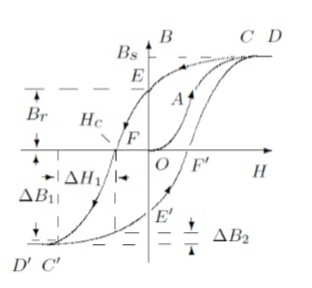
\includegraphics[width=8cm]{g1}\\
С помощью баллистического гальванометра и амперметра будем косвенно измерять зависимость индукции магнитного поля от его напряжённости. \\
Напряжённость магнитного поля \textit{Н} в тороиде зависит от тока, текущего в намагничивающей обмотке:
    $$H = \frac{N_{T_0}}{\pi D}I$$,
где $D$ - средний диаметр тора, $N_{T_0}$ - количество витков.\\
Изменение поля приводит к изменению потока магнитной индукции Ф в сердечнике, в измерительной обмотке возникает ЭДС индукции, через гальванометр, в свою очередь, протекает импульс тока, изменяется положение рамки и, следовательно, зайчика. Окончательно (определив также баллистическую постоянную гальванометра, проведя измерения с соленоидом) для изменения магнитной индукции в сердечнике тороида получаем:
$$\bigtriangleup B = \mu_0 N_c \frac{N'_c R d_c^2 \bigtriangleup I_c \bigtriangleup x}{N' R_c d^2 l_c \bigtriangleup x_c}$$
где $R$ - полное сопротивление измерительной цепи тороида, $d_C, d$ - диаметр поперечного сечения соленоида и тороида соответственно,  $N_c$ - число витков пустотелого соленоида, $N'_c$ - число витков короткой измерительной катушки $l_C$ - длина соленоида, $\triangle x_c$ - отклонение зайчика при работе с соленоидом, $\triangle x$ - отклонение зайчика в эксперименте.
\section{Экспериментальная установка}
\subsection{Схемы}
Детальная схема измерений петли гистерезиса представлена на рисунке ниже:\\
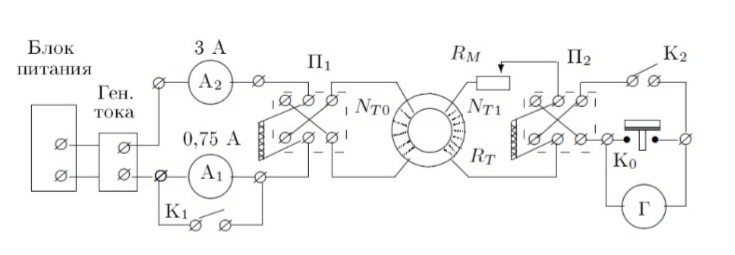
\includegraphics[width=12cm]{g2}\\
К блоку питания подключен специальный генератор, позволяющий скачками менять токи в намагничивающей обмотке.\\
Ток в намагничивающей обмотке измеряется амперметром. Переключатель П1 позволяет менять направление тока в первичной обмотке. Чувствительность гальванометра Г во вторичной цепи можно менять с помощью магазина сопротивлений $R_m$. Ключ К2 предохраняет гальванометр от перегрузок и замыкается \textit{только на время измерения отклонений зайчика}. Ключ К0 служит для мгновенной остановки зайчика. Переключатель П1 позволяет менять направление тока в первичной обмотке. Переключателем П2 можно изменять направление тока через гальванометр. Ток в намагничивающей обмотке измеряется амперметрами А1 и А2 с разными пределами измерения.\\
Схема установки для калибровки гальванометра:\\
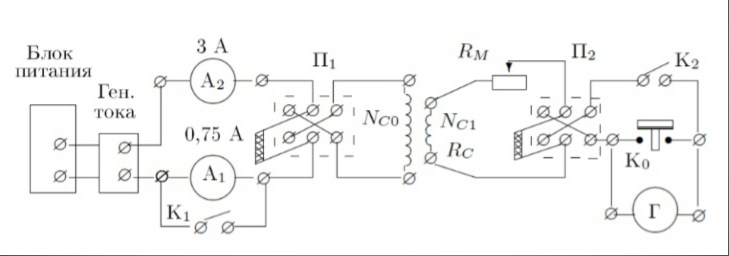
\includegraphics[width=12cm]{g3}\\
После снятия петли гистерезиса необходимо размагнитить сердечник, подключив его к цепи переменного тока, постепенно снижая его амплитуду. Только затем следует приступать к снятию основной кривой намагничивания.\\
\subsection{Размагничивание образца}
Чтобы снять начальную кривую намагничивания, нужно предварительно размагнитить образец. Для этого тороид подключается к цепи переменного тока:\\
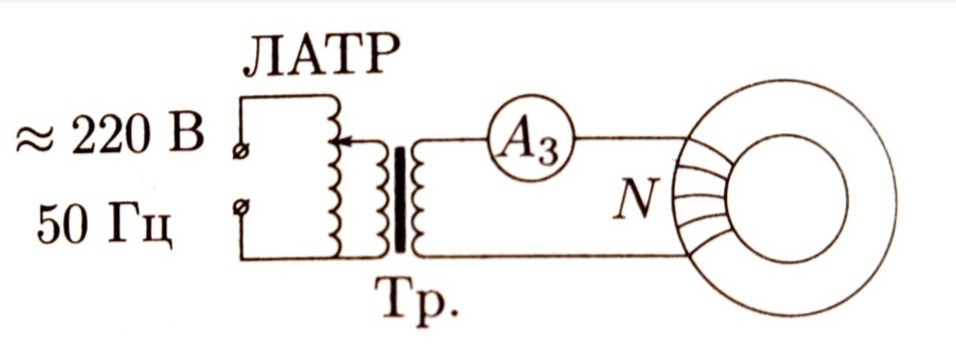
\includegraphics[width=6cm]{g4}\\
При уменьшении амплитуды тока через намагничивающую обмотку от тока насыщения до нуля характеристики сердечника В и Н <<пробегают>> за секунду 50 петель всё меньшей площади и в итоге приходят в нулевую точку.\\
\subsection{Исследование петли}
Измерения начинаются с максимального тока. Переключая тумблер генератора, следует фиксировать ток, соответствующий каждому положению тумблера, и отклонение зайчика $\triangle x$, соответствующее кажому щелчку тумблера.\\
\section{Ход работы}
1) Занесём все параметры установки в таблицу:\\
\\
\begin{tabular}{|l|l|l|l|l|l|l|l|}
\hline
$N_{T0}$ & $N'$ & $N_{c0}$ & $N_{c1}$ & D & $d_{T}$ & $d_{c}$ & $l_{c}$ \\
\hline
1750 витков & 300 витков & 825 витков & 435 витков & 0,1 м & 0,01 м & 0,07 м & 0,8 м\\
\hline
\end{tabular}\\
\\
2) Подготовив к работе экспериментальную установку, снимем зависимость величины скачка $\triangle x$ от величины силы тока в цепи $I$. Пройдём по всей петле гистерезиса, результаты занесём в таблицу.\\
Максимальное значение тока $I_{max} = 1,467$ А, $\sigma_{I_{max}} = 0,001$ А. Тумблер генератора состоит из 13 делений, соответственно, поделив макисмальное значение тока на 13, можем найти величину тока для каждой из позиций тумблера.\\
Снимем данныке для начальной кривой намагничивания:\\
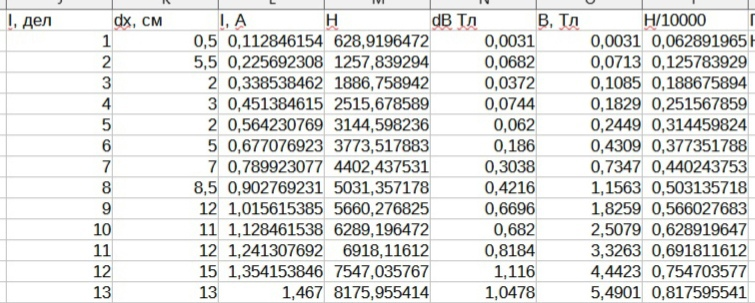
\includegraphics[width=16cm]{g9}\\
Данные для петли гистерезиса:\\
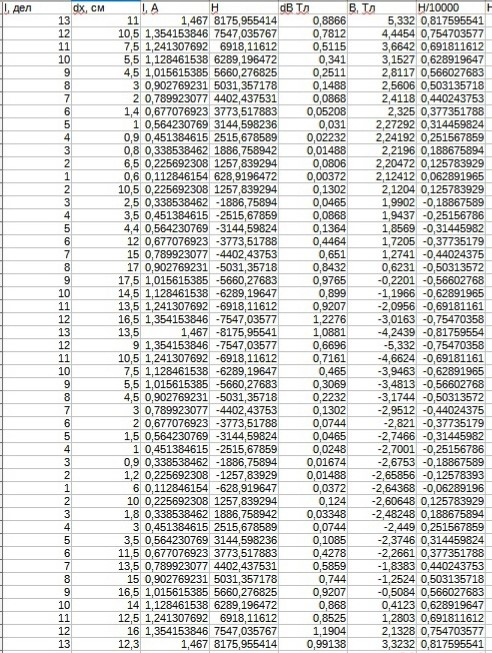
\includegraphics[width=18cm]{g8}\\
По полученным данным найдей экспериментальную зависимость B(H) и построим график:\\
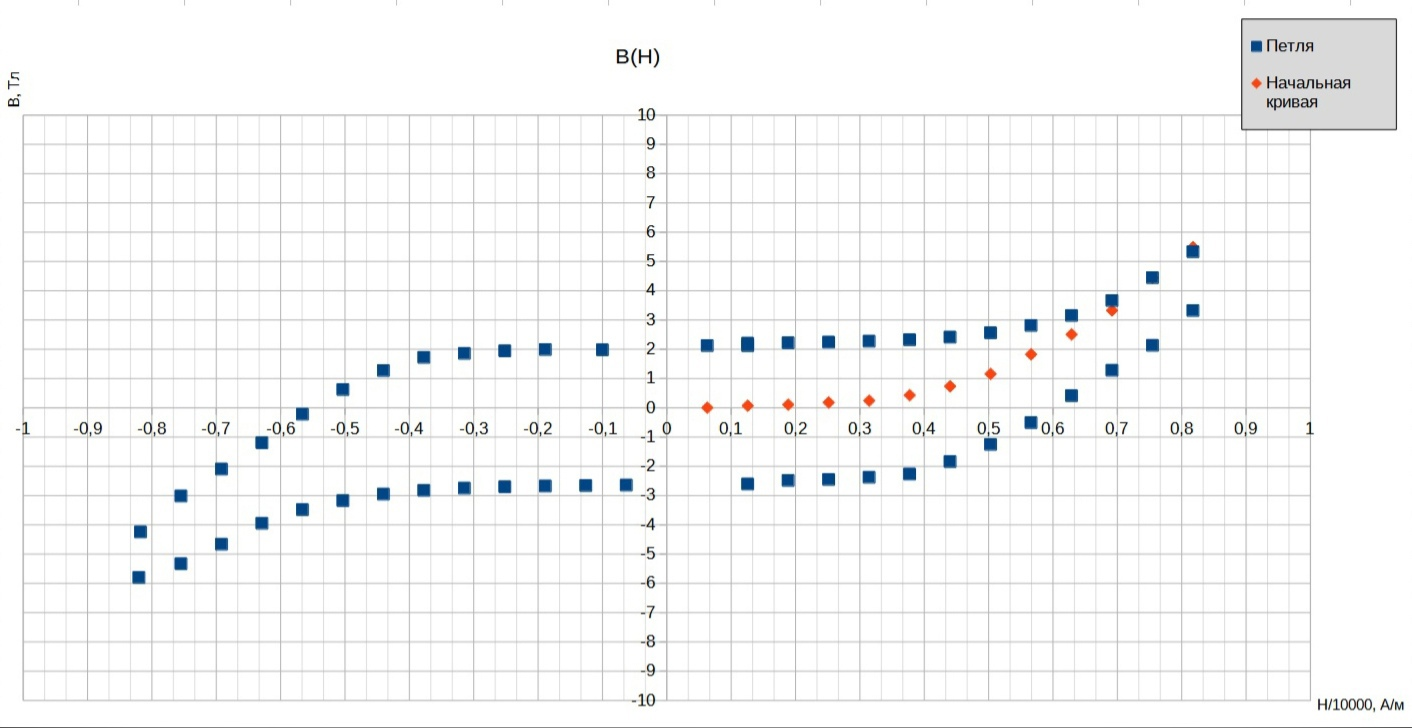
\includegraphics[width=18cm]{g5}\\
По наклону начальной кривой намагничивания определим максимальное значение дифференциальной магнитной проницаемости $\mu_{diff}$. А также некоторые другие величины:\\
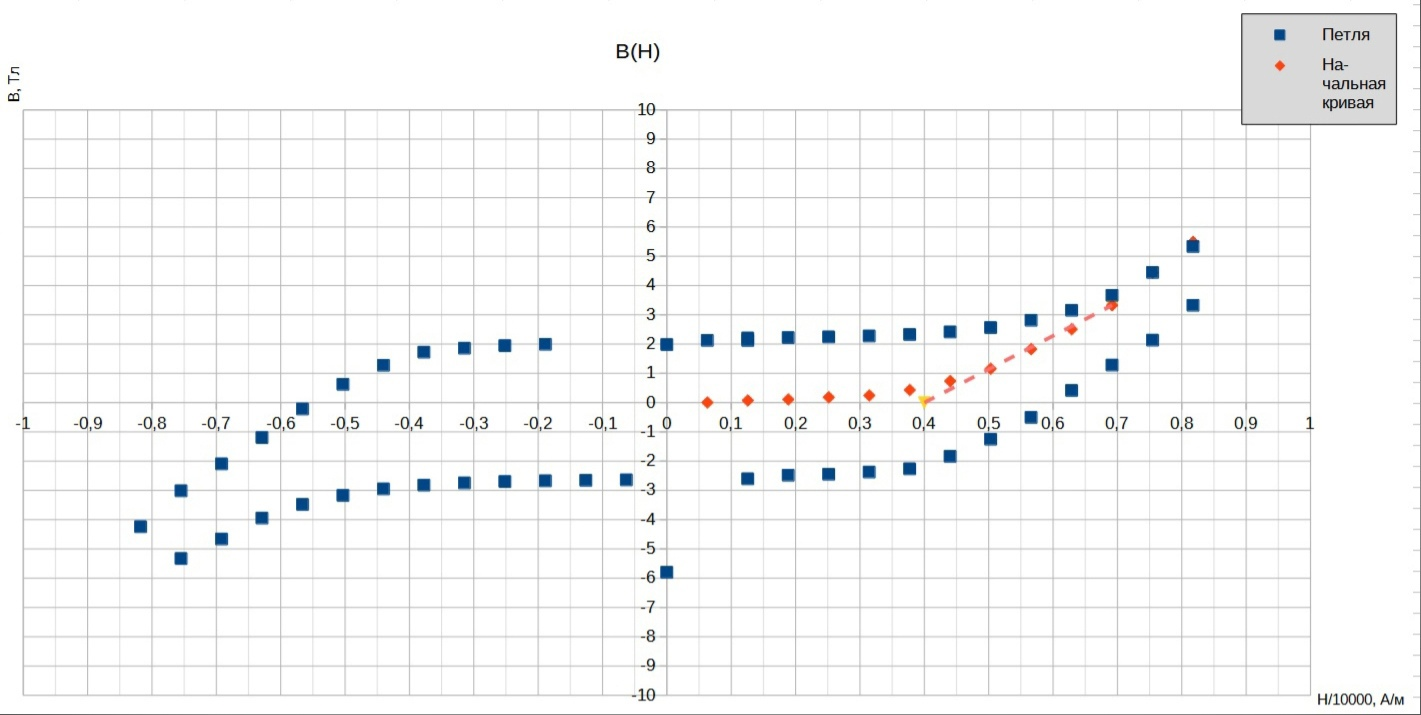
\includegraphics[width = 18cm]{g6}\\
\begin{tabular}{|l|l|l|l|}
\hline
остаточная индукция & коэрцитивное поле & индукция насыщения & дифф. магн.проницаемость\\
$B_r$ & $H_c$ & $B_s$ & $\mu_{diff}$\\
\hline
$2,0 \pm 0,2$ Тл & $0,53\cdot10000 = 5300 \pm 500$ А/м & $5,3 \pm 0,5$ Тл & $\frac{1}{\mu_{0}}\frac{dB}{dH} \approx 881 \pm 22$ \\
\hline
\end{tabular}
\section{Вывод}
В ходе данной лабораторной работы мы исследовали кривую намагничивания стали с помощью баллистического гальванометра.  Построенный график представляет собой симметричную петлю гистерезиса, что соответствует теории ферромагнетизма.\\
\begin{enumerate}
		\item 
			Вычислили коэрцитивную силу $H_c = 5300\,\pm\, 500$ А/м;
		\item 
			Определили остаточную индукцию: $B_r =2,0\,\pm\,0,2$ Тл и индукцию насыщения $B_s = 5,3\,\pm\, 0,5$ Тл;
		\item
		Определили индукцию насыщения: $B_s = 5,3 \pm 0,5$ Тл;
		\item
			Рассчитали максимальную дифференциальную магнитную проницаемость для начальной кривой намагничивания: $\mu = 881 \, \pm \, 22$;
	\end{enumerate}
Из-за того, что материал ферромагнетика неизвестен, сравнить полученные результаты с табличными не получится. Можно лишь прикинуть, что коэрцитивная сила по порядку совпадает с показаниями магнитожестких ферромагнетиков, а индукция насыщения оказалась завышенной в два раза. Можно предположить, что такие погрешности связаны с неточным определением отклонения зайчика - на глаз, даже в замедленной съемке, определить отклонение было сложно.\\
\end{document}